%%%%%%%%%%%%%%%%%%%%%%%% CAB432 Group Report %%%%%%%%%%%%%%%%%%%%%%%

%BEGIN_FOLD
% Disclaimer: You HAVE to use this. This is a not simple starting point, all libraries and titles were recreated for fit group Assignment, same way it was in EGB342. If something does not work... Well, you all know who to blame.

% This sets the style of the document, you can use different built in styles, create your own .cls files or download ones from the Internet. This one is fairly standard to use
\documentclass[12pt]{article}
\usepackage[natbibapa]{apacite}


%%%%%%%%%%%%%%%%%%%%%%%%%%%%% Packages %%%%%%%%%%%%%%%%%%%%%%%%%%%%%%

% This package is handy for captioning figures, you can set caption style here as well
\usepackage[font={small,it}]{caption}
\usepackage[a4paper, portrait, margin=0.8in,top=2cm,bottom=2cm,]{geometry}
\usepackage{bigstrut}

% This is important for position images as latex will put your image where it best fits unless you tell it otherwise
\usepackage{float}
\usepackage{wrapfig}

% If you want images this is necessary
\usepackage{graphicx}
\usepackage{subcaption}
\graphicspath{{./images}}
\usepackage{hyperref}
\usepackage{color}

\usepackage[table]{xcolor}% http://ctan.org/pkg/xcolor
\hypersetup{colorlinks=true}
\hypersetup{linkcolor=blue}
\newcommand\PlaceText[3]{%
\begin{tikzpicture}[remember picture,overlay]
\node[outer sep=0pt,inner sep=0pt,anchor=south west] 
  at ([xshift=#1,yshift=-#2]current page.north west) {#3};
\end{tikzpicture}%
}
% You can use this to set your margin size
%\usepackage[margin=25mm]{geometry}

% Allows you to do things such as headers and footers
\usepackage{fancyhdr}

% This needs to be in here if you want to set up your document with more than one column in sections 
\usepackage{multicol}

% Here are a few packages that help with formatting equations, you may not need to use this but I find align* from amsmath particularly useful
\usepackage{amsmath,amssymb,amsthm,textcomp,amsfonts,amsthm,mathrsfs}
\usepackage{xparse}% http://ctan.org/pkg/xparse
\NewDocumentCommand{\ceil}{s O{} m}{%
  \IfBooleanTF{#1} % starred
    {\left\lceil#3\right\rceil} % \ceil*[..]{..}
    {#2\lceil#3#2\rceil} % \ceil[..]{..}
}

% Enhances Latex`s cross referencing
\usepackage{cleveref}
\usepackage{hyperref}
\hypersetup{colorlinks=true}
\hypersetup{linkcolor=blue}

\usepackage{physics}
\usepackage{gensymb}
\usepackage{mathrsfs}

% Also not necessary but I find it handy when formatting arrays and matrices
\usepackage{array}
\usepackage{xfrac}
\usepackage{enumitem}

%% These packages you`ll need to download a .sty file before you can use

% This allows really nice formatting for MATLAB code.
\usepackage[numbered,framed]{mcode}
\usepackage{mathrsfs}
\usepackage{hyperref}
\hypersetup{colorlinks=true}
\hypersetup{linkcolor=blue}

\usepackage{physics}
\usepackage{gensymb}

%% Feel free to add any more packages you want!!!
\usepackage{indentfirst}
\usepackage{parskip} 
\setlength\parindent{0pt}
%\setlength{\parskip}{1cm plus4mm minus3mm}
\usepackage{csquotes}
\usepackage{mathtools}
\newcommand{\Lim}[1]{\raisebox{0.5ex}{\scalebox{0.8}{$\displaystyle \lim_{#1}\;$}}}
\usepackage{wrapfig}
\usepackage{tabularx} % in the preamble

%%%%%%%%%%%%%%%%%%%%%%%%% Setup the document %%%%%%%%%%%%%%%%%%%%%%%%

\lstset{basicstyle=\scriptsize\ttfamily,breaklines=true}
\renewcommand{\thesubsection}{\thesection.\arabic{subsection}.}

\renewcommand{\thesubsubsection}{\indent \roman{subsubsection}}

\numberwithin{equation}{section} % Number equations within sections (i.e. 1.1, 1.2, 2.1, 2.2 instead of 1, 2, 3, 4)
\numberwithin{figure}{section} % Number figures within sections (i.e. 1.1, 1.2, 2.1, 2.2 instead of 1, 2, 3, 4)
\numberwithin{table}{section} % Number tables within sections (i.e. 1.1, 1.2, 2.1, 2.2 instead of 1, 2, 3, 4)

\newcommand{\horrule}[1]{\rule{\linewidth}{#1}} % Create horizontal rule command with 1 argument of height

\title{	
	\normalfont \normalsize 
	\textsc{Queensland University of Technology} \\ [25pt] 
	\horrule{0.5pt} \\[0.4cm] % Thin top horizontal rule
	\huge CAB432 - Assignment 1 \\ Mashup Project \\ % The assignment title
	\author{ Marat (Matt) Sadykov \small n9312706 \\ \\ Tutor: Jacob Marks \small \underline{marksj@qut.edu.au}}
	\date{\normalsize\today} % Today`s date or a custom date
	\horrule{2pt} \\[0.5cm] % Thick bottom horizontal rule
}

% Headers and footers
\pagestyle{fancy}
\fancyhf{}
\rhead{Mashup Project Report}
\lhead{CAB432 Cloud Computing}
\cfoot{Marat (Matt) Sadykov}
\cfoot{Page \thepage}
\cfoot{n9312706}

%END_FOLD
%%%%%%%%%%%%%%%%%%%%% Begin the Actual Document %%%%%%%%%%%%%%%%%%%%%
\begin{document}
\maketitle
\newpage
\tableofcontents
\newpage
%===================================================%
%													%
%============ Section 1 Introduction ===============%
%												    %
%===================================================%
\section{Introduction}	
%	\begin{enumerate}
%		\item Overall mashup purpose and description (1-2 Paragraphs)
%		\item List of service and data APIs to be utilised. Short description of API (1 paragraph)
%	\end{enumerate} error made int

		The aim of this project to provide users with some comfortable environment to plan their journeys. This planner will use one of the following API\footnote{Names contain hyperlinks to the resources. Feel free to click}: 
		
		\begin{itemize}
			\item \href{https://developers.google.com/maps/documentation/}{Google Maps}
			\item \href{https://hackathon.expedia.com/docs/public/api/Flights Overview/}{Expedian} with \href{https://api.flightstats.com/flex/flightstatus/rest/v2/json/route/status/}{Flightstats} combined for one purpose.
			\item \href{https://developers.webcams.travel/\#webcams/list}{Webcam}
		\end{itemize}    
		A user will be able to choose a destination, view closes and cheapest flight information and makes a decision based on a picture from realtime webcameras (Maybe it is not as pretty, but it will give right feeling regarding destination). First and the important part is an interactive map, provided by Maps services. It will allow a user to change view between satellite and geographic, zoom in to view details and help to extract geographic locations. Next is the webcam, which produces some images or short video streams on some of the sights of the area. Moreover, the Main part is quick information on the closest flight regarding price, time and journey. The first experiment version located in the Appendix.    

	\subsection{World Map}	
		The foundation for weekend planer environment is continental Map. Gladly, there is a high chance of finding a right Map provider. Two global websites, whose work offers an API for use cases are Google Maps and Yandex. If first is the global giant, who existed in the worldwide market for a while, second has the most popularity in Russian. Both of them will serve the primary purpose very well: establish a right environment for integrating other API. Besides, both services provide an excellent API to extend the scope of the current project. \\
		
		As a result, the Google Map~\cite{noauthor_google_nodate} API provided a good environment, with a way presented in Figure~\ref{fig:gmaps}. To locate a particular area, the server has to receive a centre point of the map with longitude and latitude. Besides, API provides a good drawing environment, which allows places some images on top of the map, draw markers or lines from one location, to another. As a scope of this unit, a working environment will be stick to Australia.
		
		\begin{figure}[H]
			\centering        
			\includegraphics[width=0.7\textwidth]{images/google-map}
			\caption{Google Maps API at 54 54 longitude and latitude.}
			\label{fig:gmaps}
		\end{figure}
		
	\subsection{Flight Management}	
		In the process of gather information about the possible flight tickets, the project has potential problems, regards to context. Since the beginning of the project, the request for API keys may take longer than expected. Such services like Expedia~\cite{noauthor_expedia_nodate} provides some flight information, which may be used to gather closest flight information about time, prices, airports. Obtaining this information may become a trickier process. For example, if there will be no alternatives discovered, the best solution in this situation will be parsing web page with flight information. However, this approach goes beyond the scope of the assignment, and it may prove itself as a good, but not easy, alternative.\\
		
		As a result, plans were achieved using Flightstat~\cite{noauthor_flightstats_nodate} API in combination with Expedia. In order to produce a request which can be handled by flight API, there was a need in creating a request in particular form. In this situation, Expedia was able to provide absolute returns based on the name of the city, as an example, the code below represents two predefined messages for requests. In some situation, during the development process, Expedia refused to give the response, that is why the code contains some predefined cities, to avoid error possibility and not interrupt the user. Figure~\ref{fig:depar} provides an example of the flight from Main City\footnote{The one which user picked as starting point} to the destination.
		
		\begin{lstlisting}
			function def_(name) {
			
				if (name == 'brisbane') {
					return {
						displayName: '<B>Brisbane</B>, Queensland, AU',
						fullName: 'Brisbane (and vicinity), Queensland, Australia',
						lastSearchName: 'Brisbane, Queensland, Australia',
						shortName: '<B>Brisbane</B>, Queensland, AU',
						coordinates: {lat: '-27.458819',  long: '153.103613'},
						airport: 'BNE'
					};
				}
				
				if (name == 'sydney') {
					return {
						displayName: '<B>Sydney</B>, New South Wales, AU',
						fullName: 'Sydney (and vicinity), New South Wales, Australia',
						lastSearchName: 'Sydney, New South Wales, Australia',
						shortName: '<B>Sydney</B>, New South Wales, AU',
						coordinates: {lat:  '-33.86757', long: '151.20844'},
						airport: 'SYD'
				};
				...
				...
			}
		\end{lstlisting}
		\begin{figure}[H]
			\centering        
			\includegraphics[width=0.7\textwidth]{images/departure}
			\caption{Departure flights from Brisbane to Perth.}
			\label{fig:depar}
		\end{figure}
	\subsection{Location Explorer}
		To gather information unusually and present in on top of maps webcam service will be used. Generally, it contains Library of open web cameras located around the world. Instead of gathering all possible sources, webcam includes all of them in one place. It will allow extracting at least images, which were made very recent to a user request. An example of how data can be collected is displayed in Figure~\ref{fig:webcam}. \\
		
		As a result of hard work with Webcams~\cite{noauthor_webcams.travel_nodate} API, it was possible to integrate a real-time video playthrough, fresh within 5-15 minutes. In case if need, streams can be switched to Day, Month or Year in a minute. Video Players also includes information about the provider, link for connection and script for embed, in addition to full-screen view. Figure~\ref{fig:webCam-adel} refers to their view~\footnote{Nothing inspires more than eye dropping over someone's life or an entire city.}.
		
		\begin{figure}[H]
			\centering        
			\includegraphics[width=0.5\textwidth]{images/webcam-adel}
			\caption{Departure flights from Brisbane to Perth.}
			\label{fig:webCam-adel}
		\end{figure}
\newpage		
%===================================================%
%													%
%============ Section 2 Use Cases ==================%
%												    %
%===================================================%
\section{Use Cases}
	\subsection{Trip Planner}
		The main expected advantage of this service is plan trips to another city on one Map, instead of planning on the official website, comparing each ticket one by one. This comparison gives user possibility select option flexibly, and choose several places and time.
		
		\begin{figure}[H]
			\centering        
			\includegraphics[width=0.7\textwidth]{images/Google-web}
			\caption{Departure flights from Brisbane to Perth.}
			\label{fig:webCam}
		\end{figure}
		\begin{figure}[H]
			\begin{subfigure}[b]{0.52\textwidth}
				\centering
				\includegraphics[width=\linewidth]{images/flight-ad}
				\caption{Flights to Adelaide.}
				
			\end{subfigure}
			\begin{subfigure}[b]{0.52\textwidth}
				\centering
				\includegraphics[width=\linewidth]{images/flight-sd}
				\caption{Flights to Sydney.}
				
			\end{subfigure}
			\caption{Choosing most efficient flight.}
		\end{figure}
	\subsection{Exploring area with cameras}
		Web cameras spread around cities all other the place. Some of them may contain tedious traffic exploration, another some beautiful views. Comparing to high-quality images on other services, webcam takes real-time shoots. The original intention is to allow the user to plan short weekend trips~\footnote{There is no better way to make a decision rather take a small pick into a city of destination.}.
		\begin{figure}[H]
			\centering        
			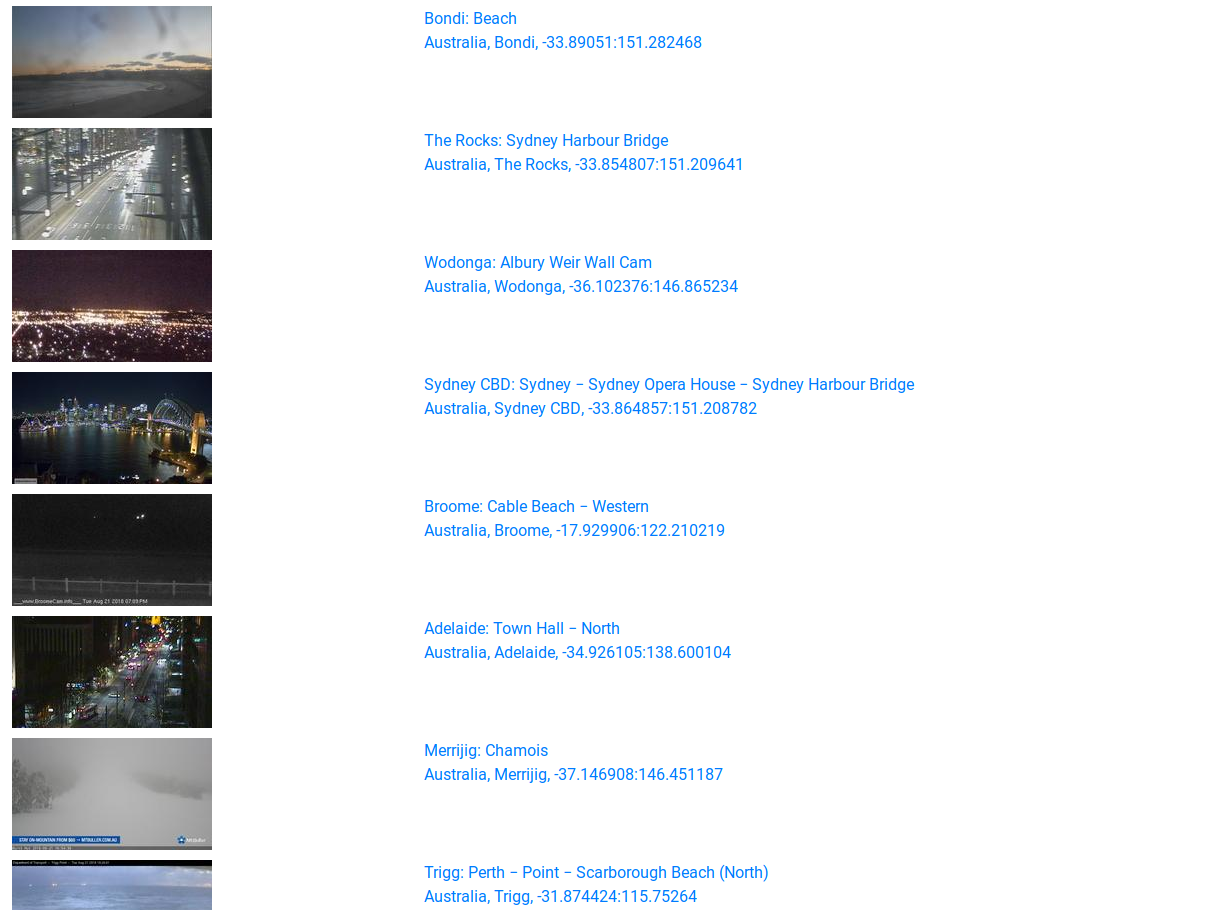
\includegraphics[width=0.7\textwidth]{images/webcam}
			\caption{First test print with API use.}
			\label{fig:webcam}
		\end{figure}
		By choosing one cities, he can visualise video of current situation in predefined area.
		\begin{figure}[H]
			\begin{subfigure}[b]{0.52\textwidth}
				\centering
				\includegraphics[width=\linewidth]{images/webcam-ch}
				\caption{Choose from server.}
				
			\end{subfigure}
			\begin{subfigure}[b]{0.52\textwidth}
				\centering
				\includegraphics[width=\linewidth]{images/webcam-lv}
				\caption{Watch live stream.}
				
			\end{subfigure}
			\caption{Webcam in Melbourne}
		\end{figure}
	
	\subsection{Exploring area with Google Maps}
		The usage of Google Maps allowed several map manipulations. One of them is changing overall map view to satellite. With zooming, the map gets added with extra details such as street names, or locations of interest, including shops, restaurants and more. Besides, Google provided a street view, which means a person can explore areas as a living virtual being. Some people may find this feature suitable for planning.
		\begin{figure}[H]
			\centering        
			\includegraphics[width=0.7\textwidth]{images/map-toss}
			\caption{Pick location to explore with Google.}
			\label{fig:toss}
		\end{figure}
	\subsection{Weekend planner}
		In addition to flight management and camera exploration, some \textbf{the Maps services} can be used to make decisions on sight. For example, explore the streets a destination in a particular city, without moving to another Map view. \\
		In addition to this stage of the project, final goal after implementing the server side of the project is to allow the possibility of integration this web application into Linux GNOME Desktop environment. With this opportunity, the user will be free from the browser and will be able to decide weekday workflow. It will allow storing some information of the user on the computer, instead of some server login/password way.
		\begin{figure}[H]
			\centering        
			\includegraphics[width=0.7\textwidth]{images/map-explore}
			\caption{Google satellite view on locations of interests.}
			\label{fig:map-satel}
		\end{figure}	
		
%===================================================%
%													%
%============ Technical Breakdown===================%
%												    %
%===================================================%
\section{Technical Breakdown}	
%	\begin{enumerate}
%		\item A clear division between Server, Client and Cloud.
%		\item  a mock-up of your application page		
%	\end{enumerate} 
	The image below~\ref{fig:break} represents the first and last structure breakdown of the current project. Arrow indicates application communication on client site, then dot arrows indicate web request and response. The blue connection between API and cloud services are constant communication to provide service.
	\begin{figure}[H]
		\centering		
		\includegraphics[width=\textwidth]{images/Breakdown}
		\caption{First structure Breakdown.}
		\label{fig:break}
	\end{figure}
	
		
\newpage
\section{Client}
%	Using only GET. Based only everything with Map. Passing all videos, and mnarking places. Then asking for flight, using click. After requesting specific city, GET post send to server and server makes response to Flight. Basically, public folder responsible for client side. \\
%	Client also uses async for speeding up process of requsting cities	\\
%	Google Overlay functions for implementations/	 \\
	
	At the loading page stage, a client is come up with Google Loaded Map, with predefined cities and their airports. First initial travelling location preallocated as Brisbane. Also, the user gets provided with the first images from the webcam, from which it is possible to view the full video. They get linked to dot markers of the cities in Australia. Those templates are build using Embedded JavaScript (.ejs) located in views directory. Besides, the similar window is applied for error message. After picking locations on the map, they get handled by JQuery and processed on the server side.
	To process each city to extract information about airports locations a way of sending asynchronous requests was used~\cite{mcmahon_async_2018}. It allowed to speed up the process of drawing the web page. \\
	
	After choosing a location to get flights from, the client will send the location of choice to server and server will form a proper request to flights management and return in proper view. Closest available flights within a day will be displayed. The user is also able to change the central city of departure, to any other with radio buttons. \\
	
	As soon as the user click any buttons which shows a pop window, another fading layout to keep out of interaction with everything else.
	
	All request are send using GET requests, this way it is better to focus all effort on the server side and keep the client out of complicated code\footnote{Except async.js - I found no better way to approach it.}
\section{Server}
	Server processes requests from the client, provides a first map page, and additional information per request. It also sends 404 page, if for some reason Map gets unavailable. In addition to error messages, if the server is in the process for extracting information, the user receives loading screen. As prior of tests, loading did not take longer than 3 seconds. \\    
	
	Server process requests from a user by adapting them into proper one to send with API posts. Upon their feedback, they are brought to visible form and presented on the client side. Regarding the flights - this strategy works well. However, video feedback from webcam gets processed much similarly. Instead of downloading a video to the server and showing to a user, the client receives a link to video stream straight from webcam and plays inside the browser. Such an approach removes need in filtering callbacks, does not store unnecessary unused information and saves the user from loading time. \\
	All API information, the configuration for the server, API requests for each service and their keys get stored inside the app folder. Upon need, they get called from js files. This way the user will not be able to get access to some private server information. \\
	File architecture in the project presented below. The app folder contains API used for requests, Views - pages for drawing and Public - A view for a browser with JQuery and CSS files. \\
	
\section{Docker}
	All instructions how to use Docker file attached in the README.md file with the application and report.\\
	Generally, Docker container used for simple deployment of the project any type server based machine. For the sake of time for building, the container gets uploaded to DockerHub repository. In order to download and deploy it, following command is enough~\footnote{Nickname of the user has nothing personal. Another simple way to remember logins combined with the past.}: \\
	\begin{lstlisting}[language=bash]
	docker run --name Assignment1 -p 8000:3000 -i -d -t smugglersmr/weekends-pl
	\end{lstlisting}
	Docker build file uses a node v8 as a base ground for the project. After installing additional application are going to be installed to simplify the debugging process. After moving all files, main port 80 going to be exposed for connection. After it, every request addressed to port 8000 will be reallocated to Docker container. After running image, there is no need for additional commands to start.\\
	\begin{lstlisting}[language=Python]
	# Set initial image to ubuntu
	FROM node:8
	# Author
	LABEL maintainer="Smuggler"
	
	# Updating
	RUN apt update && apt install -y \
	build-essential \
	curl \
	dialog \
	git \
	mc \
	net-tools \
	tar \
	vim \
	wget
	
	# copy the app
	ADD /app /app
	
	# expose
	EXPOSE 80
	
	# Default directory
	WORKDIR /app
	RUN npm install
	CMD [ "npm", "start" ]	
	\end{lstlisting}

\section{Difficulties}
%	Switch between satellite and geographic considered ti be useless. \\
%	Processing went slow, so aditional script from async was used to process connections. \\
%	Some bugs were adressed differently, with small delais and pauses during the run.
	
	This section is much harder to write than it appears, and the reason behind it is apparent. At first, you are trying to approach the difficult problem, and when you are finding solutions and it works, you starting questions yourself what was so difficult in the first place. \\
	
	For particularly this king of Cloud Computing I found it challenging to convert coordinates into latitude and longitude to apply them for Map. And certain problems with it.  Most of the time I used projects which were already created, this one was the first which I developed from nothing. Maybe it could be helpful to use better templates like a pug, but I learned about it too late. API like Maps had some issues with the building, which was hard to debug. As a result, the solution behind it was adding a small time delay. Those kinds of problems not easy to approach when you can't form a proper request to Uncle Google for a solution. \\
	I interfered with a problem passing certain information from one file to another. Understanding the logic which deriving yourself brings a new perspective for the code approach. \\
	
	Getting a price list from flights API was not an easy task, none had a will to share this opportunity freely. It could be another useful implementation to allow a user to buy those tickets or calculate prices on the way. In combinations of hotels, journey planner and other useful API, this project could become a far exciting practice that I planned initially.
	
%	\subsection{More API than necessary}
%		Design followed minimalistic approach., without feeding too much information to a user. Markers are sticked to map with coordinates conversion to long and latitude, button exists as another div object. \\
%	\subsection{Asynchronic request}
\section{Future work}
	\subsection{Gnome Integration}
		The idea to use Gnome integration considered to be irrelevant as no additional marks are going to be provided for trials. However the idea and desire still remain, there is still a hope for future projects. \\
		This could be another experience with Linux programming. Gnome on Linux is a GUI desktop environment, which supports different kinds of extensions. One of then is OpenWeather. The idea was to design a similar extension to use in Gnome environment, then there will be no use in Web Browser. All operation could be performed in a startup environment. Those extensions not protected from bugs and crashes, but it definitely will be an experience.
%	\subsection{Several Extra APIs}
%		Adding a cost was not an easy tasks as it required an additional API search. An extra API was already used to get information about cities. There will be no additional add.
	\subsection{More features}
%		Flight tickets ordering, cost calculation, information storage. \\
		Some additional options such as the ability to order those tickets, reliable saving information in the Computer memory with Gnome Extension, not in some web server. Besides, adding map explorer with some good locations of interests, hotel, food and journal for travels. Those options could make this extension much useful and attract more interest around people. Also, it could become more practical regarding usage.

\section{Tests}	
	\begin{tabularx}{\textwidth}{X|l|l}
		\textbf{Task} & \textbf{Outcome} & Result \\
		\hline
		Error screen & error.ejs applied & \cellcolor{green!25}DONE\\
		\hline
		Build Map with cities & Google Maps Overlay & \cellcolor{green!25}DONE\\
		\hline
		Cities choosing & Array with cities and markers & \cellcolor{green!25}DONE\\
		\hline
		Arrange flights & Expedian in combination with Flightstat & \cellcolor{green!25}DONE\\
		\hline
		Set cameras around cities & Webcames produces video stream & \cellcolor{green!25}DONE\\
		\hline
		Set Restrictions from user & Server/Client approach & \cellcolor{green!25}DONE\\
		\hline
		Safety measures for API falling & Predefined cities. No Video storage. & \cellcolor{green!10}Sort Of\\
		\hline
		Asynchronous requests handling & async.js integrated & \cellcolor{green!25}DONE\\
		\hline
		Docker establishment & Dockerfile initialised & \cellcolor{green!25}DONE\\
		\hline
		Usage of the Docker container & Container created and stored in Hub & \cellcolor{green!25}DONE\\
		\hline		
		GitHub and DockerHub & Both created as safety measure & \cellcolor{green!25}DONE\\
		\hline
		Latex Proposal and Report & Proposal and Report complete & \cellcolor{green!25}DONE\\
		\hline
	\end{tabularx}
	 \\ \\
	An example of test written for getting information from API is provided below. All test results and process of development included in Appendix below.
	\begin{figure}[H]
		\centering		
		\includegraphics[width=0.8\textwidth]{images/test-term}
		\caption{First test implementation.}
		
	\end{figure}
%===================================================%
%													%
%============Bibliography and refferencing==========%
%												    %
%===================================================%
\begin{flushleft}
	\bibliographystyle{apacite}
	\bibliography{referencing/referenceList}
\end{flushleft}

\section{Appendix}	
	\begin{figure}[H]
		\centering		
		\includegraphics[width=0.8\textwidth]{images/map}
		\caption{First test implementation.}
		
	\end{figure}
	
	\begin{figure}[H]
		\centering        
		\includegraphics[width=0.7\textwidth]{images/map2}
		\caption{First version of overview.}
		\label{fig:map2}
	\end{figure}
	
	\begin{figure}[H]
		\begin{subfigure}[b]{0.25\textwidth}
			\centering
			\includegraphics[width=\linewidth]{images/fl-1}
			\caption{First part.}			
		\end{subfigure}
		\begin{subfigure}[b]{0.25\textwidth}
			\centering
			\includegraphics[width=\linewidth]{images/fl-2}
			\caption{Second part.}			
		\end{subfigure}
		\caption{File structure}
	\end{figure}

	\begin{figure}[H]
		\centering		
		\includegraphics[width=0.8\textwidth]{images/Append-1}
		\caption{First test implementation.}
	\end{figure}
	\begin{figure}[H]
		\centering		
		\includegraphics[width=0.8\textwidth]{images/Append-2}
		\caption{First test implementation.}
	\end{figure}
	\begin{figure}[H]
		\centering		
		\includegraphics[width=0.8\textwidth]{images/Append-3}
		\caption{First test implementation.}
	\end{figure}
	
	\begin{figure}[H]
		\centering		
		\includegraphics[width=0.8\textwidth]{images/Append-4}
		\caption{First test implementation.}
	\end{figure}

\end{document}
